\documentclass[a4paper,11pt]{article}
\usepackage{tikz}
\usetikzlibrary{arrows}

% Unused macros removed for clarity (they were empty anyway)
% \def\onebox{...} etc.

\begin{document}

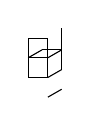
\begin{tikzpicture}
  % Draw the base rectangle (0.25 wide, 0.5 tall)
  \draw (0,0) rectangle (0.25,0.5);
  
  % Define key reference points for clarity
  \coordinate (bottom left)     at (0,0);
  \coordinate (top left)        at (0,0.5);
  \coordinate (bottom right)    at (0.25,0);
  \coordinate (top right)       at (0.25,0.5);
  \coordinate (mid left)        at (0,0.25);
  \coordinate (mid right)       at (0.25,0.25);
  
  % Horizontal line through the middle of the rectangle
  \draw (mid left) -- (mid right);
  
  % Four diagonal lines pointing upward-right from four base points
  % Each starts at a base point and goes to (x+0.175, y+0.1)
  \draw (mid left)       -- ++(0.175,0.1);
  \draw (mid right)      -- ++(0.175,0.1);
  \draw (bottom right)   -- ++(0.175,0.1);
  \draw (0.25,-0.25)     -- ++(0.175,0.1); % point below bottom right
  
  % Vertical line connecting top of diagonals to a lower point
  \draw (0.425,0.625) -- (0.425,0.1);
  
  % Horizontal line at the top of the first diagonal (from mid left)
  \draw (0.175,0.35) -- ++(0.25,0);
\end{tikzpicture}

\end{document}